%
%	Praxisbezug
%

\pagebreak
\section{Data Analysis}

\onehalfspacing

\subsection{Page Impressions}

We have completed our data exploration; now, it's time to focus on the analysis and some of the more common KPIs in web analytics and inbound marketing.

Unfortunately, wp-statistics does not offer detailed measurements for interaction or click-through rates, unlike Plausible\footnote{See \textit{Frank, C. (2021)}: Web Traffic Analysis - Predicting Blog Post Performance. \cite{previousBigData}} or Matomo; we'll need to extrapolate the data and visitor behavior from our knowledge of the site and use whatever metrics the tool offers.

Let's first look at the anatomy of the blog:

\begin{figure}[H]
\centering
\caption {Page Types}
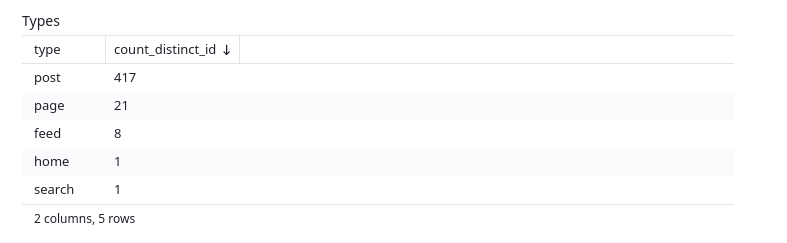
\includegraphics[width=\linewidth]{images/figure10.png}
\label{fig:pageTypes}
\end{figure}

We had 417 separate posts on the blog in early April, together with 21 utility pages, not counting the home page. The home page is where people start browsing when they do not come from a search engine or a social media reference; this could be from a bookmark or the main URL. 

The 21 pages form the top-level menu of the blog, and we will ignore them from here on. Also, we will not include the RSS Feed or the search function in our evaluation.

Let's drill down a bit and look at the page impressions by type:

\begin{figure}[H]
\centering
\caption {Impression by Page Type}
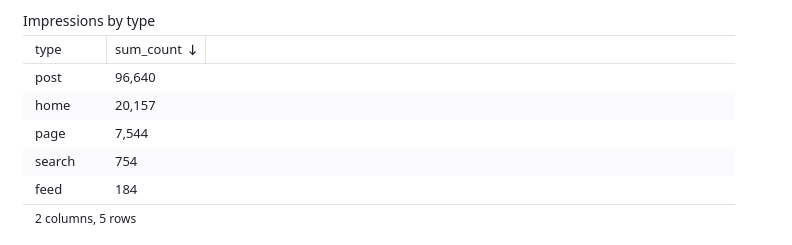
\includegraphics[width=\linewidth]{images/figure11.png}
\label{fig:impressionType}
\end{figure}

The most read items on the blog are the individual posts, which is good for us. It might not sound obvious, but if a user accesses the main page from the URL and scrolls down, we have no way of determining which of the recent posts they might have read.

For this reason, I'll concentrate further analysis on the page impressions of the posts alone and ignore the other types.

A key question for our analysis is to determine which category of posts is of most interest to our readers. We know the most-used search terms already, but we now need to see whether this is true for the actual posts. As a next step, let's try to find the top 12 most-read posts:

\begin{figure}[H]
\centering
\caption {Top Performing Posts}
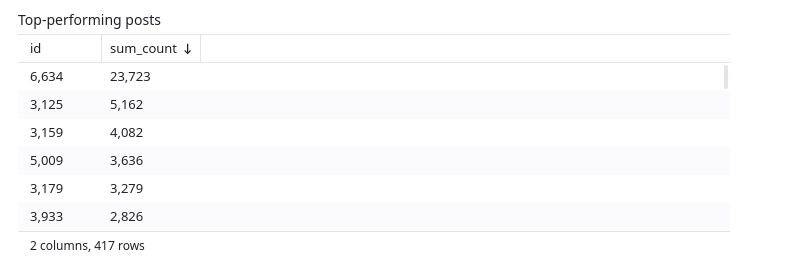
\includegraphics[width=\linewidth]{images/figure12.png}
\label{fig:topPerforming}
\end{figure}

We have the post's id, but identifying the actual posts is a bit of manual work: wp-statistics, unfortunately, records in the URI all Url-parameters, including tracking parameters such as fbclid. There's an option in wp-statistics to disable that behavior, but not retroactively. Also, wp-statistics does not record the post title itself. 

By inspecting the URL and ID, I manually created a new table which includes the actual blog title, together with its date and visits:

\begin{figure}[H]
\centering
\caption {Top Performing Posts}
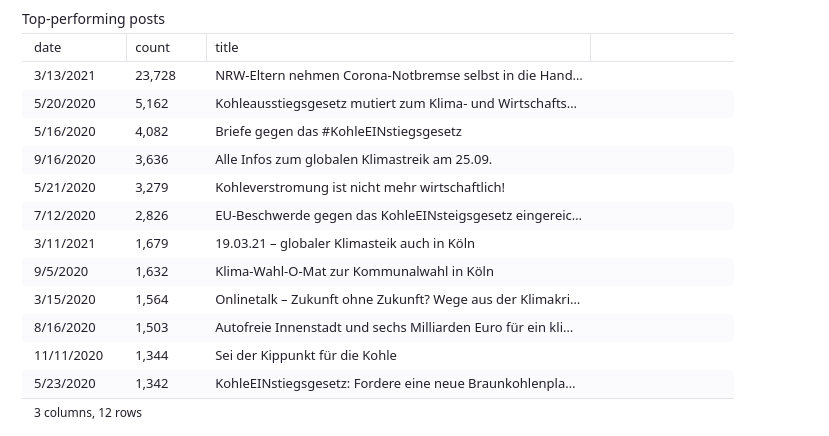
\includegraphics[width=\linewidth]{images/figure13.png}
\label{fig:manualReview}
\end{figure}

In addition to the global climate strike and local elections, content that we have identified previously from search, we can now see that the top-performing post is related to Covid-19, which is not surprising, given the severe nature of the current situation in the pandemic.

Going through the top-performing blog posts and combining this information with our results on search in the previous chapter, I was able to identify the top four content categories:

\begin{itemize}
 \item Covid-19
 \item Local election
 \item Climate strike
 \item Stop fossil fuels
\end{itemize}

The blog supports the community of climate activists in Cologne and provides the most needed and sought-after information.

\subsection{Direct Engagements through Forms}

In addition to the posts, the blog also has a contact form and a donation form. Let's have a look and find out if people are actually using them:

\begin{figure}[H]
\centering
\caption {Engagement through Forms}
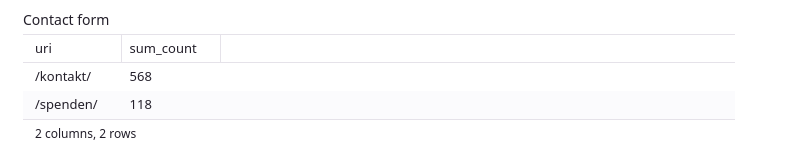
\includegraphics[width=\linewidth]{images/figure14.png}
\label{fig:engagementForms}
\end{figure}

Compared to the number of impressions on the posts, these numbers are rather low. It is most likely due to their page design, and a key takeaway for the future could be the following action items:

\begin{itemize}
 \item Redesign contact form
 \item Redesign donations
\end{itemize}

\subsection{Direct Engagement through Comments}

In addition to reading a post, WordPress allows two forms of direct engagement: pingbacks\footnote{See \textit{WPBeginner (2021)}: What is Pingback. \cite{pingBack}} and comments. 

There's one other form of interaction, trackbacks\footnote{See \textit{WPExplorer.com (2020)}: WordPress Pingbacks and Trackbacks. \cite{trackBack}}, of which we do not have any insight into.

Let's start with the pingbacks and identify the blog posts that are most referenced from other blogs:

\begin{figure}[H]
\centering
\caption {Pingbacks}
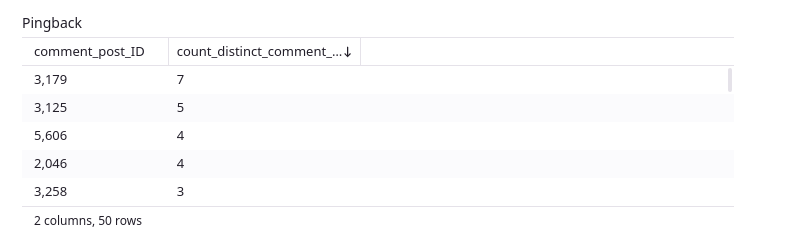
\includegraphics[width=\linewidth]{images/figure15.png}
\label{fig:pingbacks}
\end{figure}

The two most linked posts are also in the list of the dozen most-visited posts and deal with the urgent need to stop using fossil fuels:

\begin{figure}[H]
\centering
\caption {Pingback Targets}
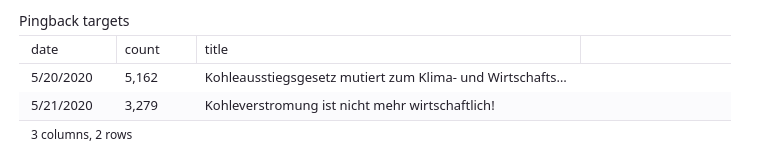
\includegraphics[width=\linewidth]{images/figure16.png}
\label{fig:pingbackTargets}
\end{figure}

With an open-pit lignite mine nearby, fossil fuels, or better the need to stop using it, is on everybody's mind, and our community seems to be a valued source for reference information.

For the final part of the engagement analysis, let's look at comments. Leaving a comment is the most active form of engagement a blog can have - there are no "Like" or "Share" buttons, to interact in any other way than reading a post the only option they have is to leave a comment:

\begin{figure}[H]
\centering
\caption {Comments}
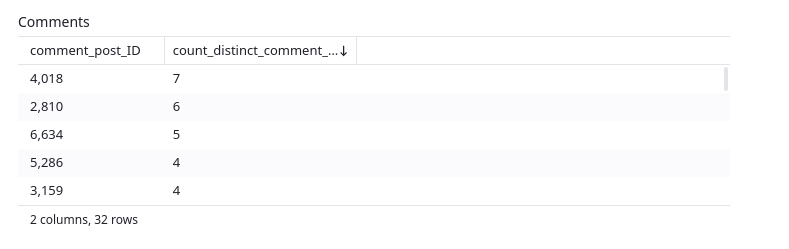
\includegraphics[width=\linewidth]{images/figure17.png}
\label{fig:comments}
\end{figure}

The two posts with the most comments are about participating in the climate accord and a lignite complaint, and the third is our most visited post on Covid-19:

\begin{figure}[H]
\centering
\caption {Comment Targets}
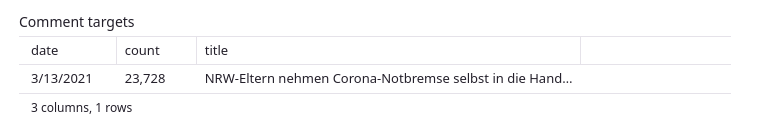
\includegraphics[width=\linewidth]{images/figure18.png}
\label{fig:commentTarget}
\end{figure}

We can again see significant engagement in our core messaging from the community. 

The blog is an integral part of our digital outreach and helps us keep the activism alive during the Covid-19 pandemic.

To finish, we'll look at multiple interactions, i.e. whether we have comments on comments:

\begin{figure}[H]
\centering
\caption {Comments on Comments}
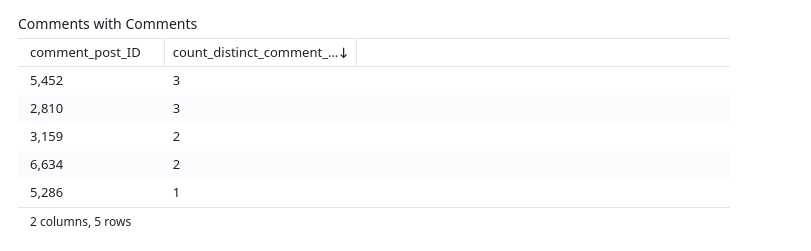
\includegraphics[width=\linewidth]{images/figure19.png}
\label{fig:commentsComment}
\end{figure}

And there are quite a few - for a blog, this is the highest form of interaction: A post that's not only read and commented on but where the readers also have replied to a previous comment.

\subsection{Improving Analytics}

From the analysis of the data and given the difficulties with extracting basic metrics, I think an essential task for the future will be to improve the web analytics capabilities of the blog through the use of a different tool, such as Matomo or Plausible.

In a previous paper, I have covered Plausible in more detail and compared it with other web analytics tools.\footnote{See \textit{Frank, C. (2020)}: Usefulness of open-source tools for web analytics in E-Marketing. \cite{previousPaper}} I will not go any further into details of the software itself here.

\begin{figure}[H]
\centering
\caption {Plausible}
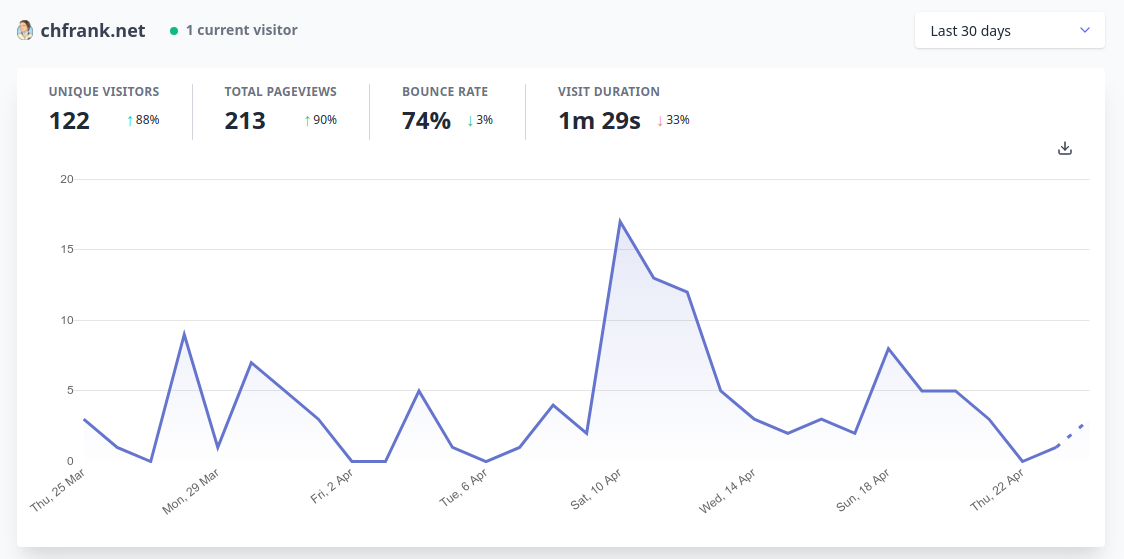
\includegraphics[width=\linewidth]{images/plausible.png}
\label{fig:plausible}
\end{figure}

In addition to a better tool for web analytics, I will also recommend the following tasks:

\begin{itemize}
 \item Paying attention to web vitals\footnote{See \textit{Sousa, B. (2021)}: Google Web Vitals best practices for single-page apps.\cite{webVitals}}
 \item Installing a caching plugin to speed up mobile access\footnote{See \textit{Crowe, A. (2021)}: WordPress Checklist. \cite{wpCachePlugin}}
\end{itemize}

\subsection{Sustaining Engagement}

From analyzing the web traffic data, we can safely deduct a couple of items:

\begin{itemize}
 \item To sustain the current level of high community engagement, we should continue our focus on local events (elections and issues around fossil fuels) and the major global crises (Covid-19 and the climate emergency)
 \item We've found out that digital activism supports offline activism and can help in combating loneliness
 \item To keep our communication safe and open, we need to fight hate speech, Ableism, and all other forms of negative -isms in our communication
 \item To further improve our outreach, we should implement the lessons learned above
\end{itemize}
